\begin{figure}[bth]
  \begin{center}
    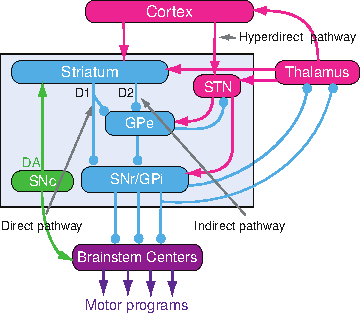
\includegraphics[width=0.9\linewidth]{ch-intro/figures/BGAnatomy}
    \caption[Anatomy of the Basal Ganglia]
    {\textbf{Anatomy of the basal ganglia.}
    STN: subthalamic nucleus;
    GPe: globus pallidus externus;
    SNc: substantia nigra pars compacta;
    SNr: substantia nigra pars reticulata;
    GPi: globus pallidus internus;
    DA: Dopamine.
    Figure slightly modified from~\cite{Grillner2016BG}.
    }
    \label{fig:intro:BGAnatomy}
  \end{center}
\end{figure}